\chapter{Implementation}

% Containing a comprehensive description of the implementation of your software, including the language(s) and platform chosen, problems encountered, any changes made to the design as a result of the implementation, etc.

\section{Languages \& Tools}\label{sec:languages-tools}
As discussed previously, the application is going to be built with Electron. As a result of this, the choice of programming languages was limited to just two; JavaScript or TypeScript. TypeScript is a relatively new language, developed by Microsoft, that adds strict typing to the traditional web programming language, JavaScript \cite{typescript}. Although the type checking provided by TypeScript is often found to lead to less bugs in software, it was decided that JavaScript should be used for this project. There are two main reasons for this decision. Firstly, TypeScript would require further learning before any implementation could be done, which would slow development of a minimum viable product (MVP). In addition, issues can be encountered if JavaScript libraries are to be used which do not have type definitions. Being able to use JavaScript for both the frontend user interface and the backend service means less context-switching and a more rapid development process.

Rather than using vanilla JavaScript, to aid in rapid development of the user interface, a Frontend JavaScript Framework was used.  There were three candidates of frontend framework: React \cite{react}, Vue \cite{vue}, and Angular 2 \cite{angular}. Vue has the smallest developer community of the three, so it was decided that the decision should be made between React and Angular 2, to ensure a good availability of supporting libraries and supporting documentation \cite{so-dev-survey}. In deciding between React and Angular 2, a number of factors were considered. React allows for extremely fast development with JSX markup, is extremely performant due to the React Virtual DOM, and encourages Functional Programming which results in code that is easy to test and highly reusable. It is largely accepted that Angular 2, as a much larger framework has a steep learning curve, which could slow down development, especially given prior experience with React. Since there are few drawbacks of using React over Angular 2, and given prior experience with using React to build large scale applications in an industrial environment, the decision was made to use React in the project to allow for rapid development using modular, reusable UI components.

In addition to the core functionality provided by React, Redux \cite{redux} was chosen as the library for application-level state management. The primary reason for choosing Redux over other React state management libraries was that its immutable state model makes for extremely simple and efficient testing, which avoids lots of time being spent on writing complex unit tests for global state, which can be better spent on writing application source code.

\subsection{Build Tools}
In addition to the core tools being used for implementation, there are a number of build steps that are required to generate an executable for the application, which are supported by a chain of build tools. The build tools used in this project consist of the following:

\begin{itemize}
  \item \textbf{Babel} is used to transpile the JavaScript from ES6, with JSX, into Electron-compatible ES5 \cite{babel}.
  \item \textbf{Webpack} is then used to bundle the transpiled JavaScript, as well as any other required assets such as images, or stylesheets \cite{webpack}.
  \item \textbf{Electron Builder} then packages the application bundles into self-contained executable Electron applications for Windows, Linux and MacOS environments \cite{electron-builder}.
\end{itemize}

Separate Babel and Webpack configurations have been created for building each of the Electron processes that form the complete application, discussed further in Section \ref{sec:electron-architecture}. An overview of the entire build process can be seen in Figure \ref{fig:build-process}.

\begin{figure}[h!]
  \begin{center}
    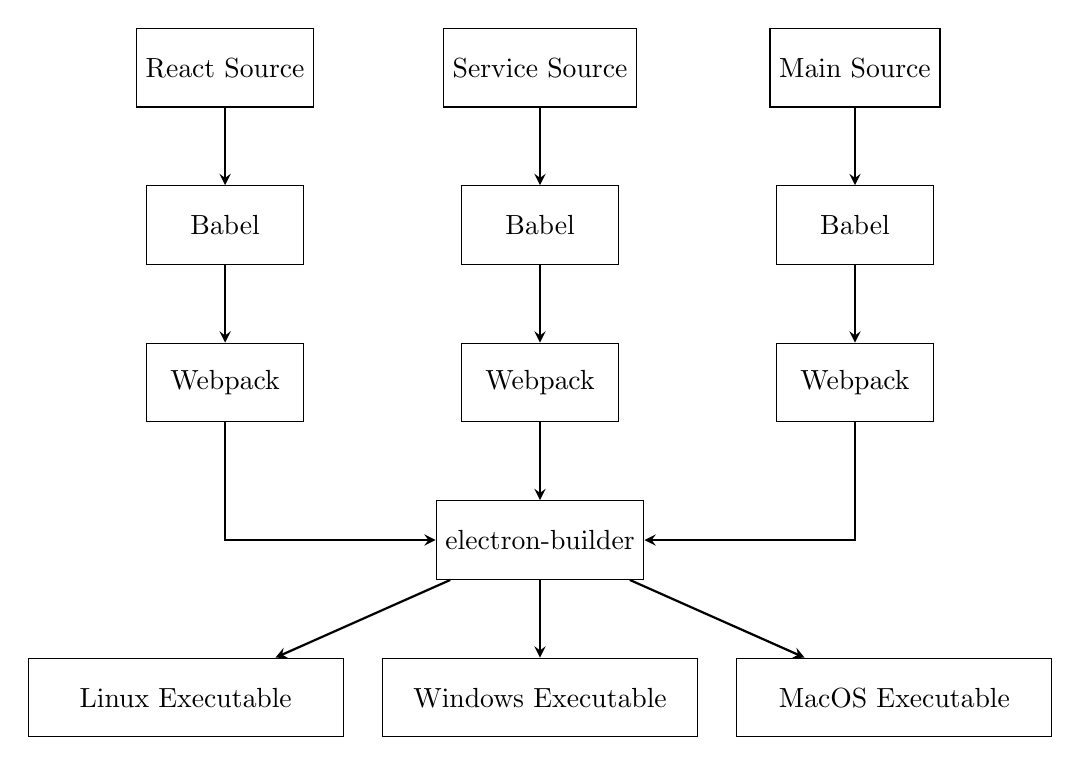
\begin{tikzpicture}[node distance=2cm]
      \tikzstyle{source} = [rectangle, minimum width=2cm, minimum height=1cm, text centered, draw=black]
      \tikzstyle{babel} = [rectangle, minimum width=2cm, minimum height=1cm, text centered, draw=black]
      \tikzstyle{webpack} = [rectangle, minimum width=2cm, minimum height=1cm, text centered, draw=black]
      \tikzstyle{electron-builder} = [rectangle, minimum width=2cm, minimum height=1cm, text centered, draw=black]
      \tikzstyle{executable} = [rectangle, minimum width=4cm, minimum height=1cm, text centered, draw=black]
      \tikzstyle{arrow} = [thick,->,>=stealth]

      \node (r1) [source] {React Source};
      \node (r2) [babel, below of=r1] {Babel};
      \node (r3) [webpack, below of=r2] {Webpack};

      \node (s1) [source, right of=r1, xshift=2cm] {Service Source};
      \node (s2) [babel, right of=r2, xshift=2cm] {Babel};
      \node (s3) [webpack, right of=r3, xshift=2cm] {Webpack};

      \node (m1) [source, right of=s1, xshift=2cm] {Main Source};
      \node (m2) [babel, right of=s2, xshift=2cm] {Babel};
      \node (m3) [webpack, right of=s3, xshift=2cm] {Webpack};

      \node (eb) [electron-builder, below of=s3] {electron-builder};
      \node (winexe) [executable, below of=eb] {Windows Executable};
      \node (linuxexe) [executable, left of=winexe, xshift=-2.5cm] {Linux Executable};
      \node (macexe) [executable, right of=winexe, xshift=2.5cm] {MacOS Executable};

      \draw [arrow] (r1) -- (r2);
      \draw [arrow] (r2) -- (r3);

      \draw [arrow] (s1) -- (s2);
      \draw [arrow] (s2) -- (s3);

      \draw [arrow] (m1) -- (m2);
      \draw [arrow] (m2) -- (m3);
      
      \draw [arrow] (m3) |- (eb);
      \draw [arrow] (r3) |- (eb);
      \draw [arrow] (s3) -- (eb);

      \draw [arrow] (eb) -- (winexe);
      \draw [arrow] (eb) -- (linuxexe);
      \draw [arrow] (eb) -- (macexe);
    \end{tikzpicture}
    \caption{Flowchart illustrating the build process}
    \label{fig:build-process}
  \end{center}
\end{figure}

\section{Application Architecture}\label{sec:electron-architecture}

\begin{figure}[h!]
  \begin{center}
    \begin{tikzpicture}
      \draw[dashed] (0,0) -- (9,0) -- (9,8) -- (0,8) node[above right, align=left] {Application Boundary} -- (0,0);
      \draw [solid] (0.5,5.5) rectangle node (main) {Electron Main Process} (8.5, 7.5);
      \draw [solid] (0.5,0.5) rectangle node (frontend) [text width=3.25cm, align=center] {Frontend\\Renderer Process} (4, 5);
      \draw [solid] (5,0.5) rectangle node (service) [text width=3.25cm, align=center] {Service\\Renderer Process} (8.5, 5);

      \draw [solid] (0,-3) rectangle node (keystore) [align=center] {OS Keystore} (9, -1);

      \node[cloud, cloud puffs=11, minimum width=3cm, draw] (cloud) at (12, 2.75) {Internet};
      
      \node[minimum width=3cm, minimum height=1cm, above of=cloud, draw=black, yshift=2cm] (imap) {IMAP Server};
      \node[minimum width=3cm, minimum height=1cm, below of=cloud, draw=black, yshift=-2cm] (smtp) {SMTP Server};

      \draw [thick,<->,>=stealth] (frontend) -- node [above] {IPC} (service);
      \draw [thick,<->,>=stealth] (6.75, 0.5) -- (6.75, -1);
      \draw [thick,<->,>=stealth] (service) -- (cloud);
      \draw [thick,<->,>=stealth] (imap) -- (cloud);
      \draw [thick,<->,>=stealth] (smtp) -- (cloud);
    \end{tikzpicture}
    \caption{Application architecture diagram}
    \label{fig:new-send-process}
  \end{center}
\end{figure}

As discussed in Section \ref{sec:high-level-architecture}, the application is being developed using Electron. This design decision brings some specific stipulations regarding the application's internal architecture. It was decided that the frontend user interface part of the application should be decoupled from the backend service component. This ensures that the code is maintainable, and it also means that if the application was to be ported to a different platform in the future, such as mobile devices, the backend could be reused with minimal modification and just connected to a new native frontend.

It was decided that the best way to achieve this decoupling in the context of an Electron application would be to utilize two different renderer processes; one for the frontend and one for the service. Electron has two different types of process: the `Main Process', and `Renderer Processes' \cite{electron-architecture}. The main process is the parent process to all of the renderer processes, and it is the only process that is able to call native GUI APIs \cite{electron-architecture}. Each renderer process has the ability to optionally display a web page inside a \verb|BrowserWindow|. Importantly, every application must have exactly one Main process but can have multiple renderer processes.

The main process contains the application UI thread, and therefore it is imperative that it is not blocked by long-running operations in order to avoid the whole application freezing until the main process becomes available again \cite{electron-performance}. With this restriction in mind, the application was architected to make use of a main process and two renderer processes; one to house the frontend React app, and one to host the backend service responsible for managing the sending and receiving of email.

These two renderer processes are able to communicate with each other using Electron's built in Inter-Process Communication (IPC) functionality, which uses `named pipes' internally to ensure fast and secure communication \cite{chromium-ipc}. The inter-process communication in Electron is implemented through the event-driven architecture that underpins much of the core Node.js API \cite{node-events}. This message-based IPC allows messages with optional data payloads to be sent between processes, and requires event listeners to be defined in the receiving process, to perform some task when messages are received.

In this project, IPC event listeners in the service renderer process are all contained in one file, for ease of maintenance, and often call methods on other objects that exist within the service, such as the \verb|MailManager|. In the frontend process, in keeping with React best practices, the event listeners are most commonly written in the \verb|componentDidMount()| method \cite{react-components} of the component that requires the data from the service. This means that the event listeners are registered as soon as the component has been mounted to the React Virtual DOM. once received, the data is often then used to update the component state by calling \verb|setState()| \cite{react-state}.

\section{Security}
One of the requirements for the application is that it must implement end-to-end encryption of messages that are being sent. This security security requirement presented a number of implementation challenges and contributed to a large amount of development time. Given that security and privacy were key motivators for completing this project, the security model of the application and its implementation is discussed in considerable detail.

\subsection{Cryptographic Algorithms}
An important technical decision that had to be made was the cipher that would be used for encryption of messages, as well as the key derivation function to be used to generate a symmetric key. The decision was taken to use the Advanced Encryption Standard, specifically AES-256, cipher since it is widely available, well documented and tested, and generally considered to be secure \cite{daemen2013design}. In addition, the `AES Instruction Set' is integrated into many processors, meaning that encryption and decryption can be carried out extremely efficiently \cite{bos2011efficient}. 

Rather than building the AES algorithm from scratch based on the specification, and risk making implementation errors that result in it being insecure, the project uses the OpenSSL implementation, via the Node.js crypto library. Since AES is a block cipher, it was necessary to choose a mode of operation to use when encrypting messages. The mode chosen was Galois Counter Mode (GCM) \cite{mcgrew2004galois} as it effectively turns the block cipher into a stream cipher and so can be used to encrypt messages of any length. In addition, this mode of operation has the added benefit of generating a message authentication tag in the same pass as encryption, to ensure integrity, giving confidence that the message has not been modified. When messages are received, the authentication tag is also present, and if the authentication tag is invalid for the received message then it is silently discarded to protect against attacks. The 256-bit encryption key is generated using the PBKDF2 algorithm, with an input password and salt, each of 64 cryptographically random bytes, and SHA512 used as a digest. The number of iterations of PBKDF2 has been set at 100,000 as a tradeoff between speed of key generation and cryptographic security. Crucially, a new initialization vector, of 128 cryptographically random bytes is generated each time a message is encrypted, to mitigate the risk of crib-dragging in a known-plaintext attack.

\subsection{Key Exchange}
One important consideration that had to be taken into account when designing the security model for the application was that groups can contain multiple users, and end-to-end encryption must be in place between all participants in a group conversation, whilst minimising computational and communication overhead as much as possible. The first implementation idea was to utilise a Diffie-Hellman key exchange to establish shared secrets between each pair of participants, which are then used to encrypt messages. Whilst this implementation would work well between two participants, in a conversation with multiple participants, every message would have to be encrypted multiple times, with the different key for each recipient, and then sent separately to each recipient. This would make message sending slower and key management would be more difficult.

To avoid this overhead, it was decided that each conversation should utilise a single `Conversation Key' which is known by all participants, and all messages within a conversation are to be encrypted and decrypted with this key using a the AES-256 symmetric cipher. There still remains the problem of ensuring that all participants receive the Conversation Key without it ever being sent across the network in plaintext.

To achieve this, asymmetric (public-key) RSA cryptography is first used to securely transport the Conversation Key between participants when a conversation is started, and then switching to faster symmetric encryption. Briefly, the client that wishes to start a new conversation will send a message to each participant requesting their RSA public key. When each of the public keys is received, the conversation key is encrypted with the public key and is sent back to the other participant. The participant then uses their private key to decrypt the message and gain access to the conversation key. The key exchange process utilises some of the message schemas defined in section \ref{sec:message-threading-model}. The sequence diagram in figure \ref{fig:security-sequence} shows the key exchange process between a group of participants.

\begin{figure}[h!]
  \begin{center}
    \begin{tikzpicture}
      \coordinate (a) at (0,-16);
      \coordinate (b) at (0,-0.5);
      \coordinate (c) at (12,-16);
      \coordinate (d) at (12,-0.5);
      \draw [dashed] (a) -- (b)node[pos=1.025,scale=1,font=\bfseries]{Alice} (c) -- (d)node[pos=1.025,scale=1,font=\bfseries]{Bob};

      \draw [densely dotted] (-1,-11.5) -- node[midway, align=center, font=\itshape]{Once Key Exchange is complete for all participants,\\encrypted messages can be sent and received} (13,-11.5);


      \draw[-{Latex[length=3mm]}] (0,-1) -- (1,-1) -- node[right,scale=1,midway]{Start Conversation} (1,-1.5) -- (0,-1.5);
      
      \draw[-{Latex[length=3mm]}] (0,-2.5) -- (1,-2.5) -- node[right,scale=1,midway]{Generate Conversation Key} (1,-3) -- (0,-3);

      \draw[-{Latex[length=3mm]}] (0,-4) -- node[above,scale=1,midway]{Request Public Key}(12,-4);
      
      \draw[-{Latex[length=3mm]}] (12,-5) -- (11,-5) -- node[left,scale=1,midway]{Generate 4096bit RSA Keypair} (11,-5.5) -- (12,-5.5);
      
      \draw[-{Latex[length=3mm]}] (12,-6.5) -- node[above,scale=1,midway]{Public Key}(0,-6.5);
      
      \draw[-{Latex[length=3mm]}] (0,-7.5) -- (1,-7.5) -- node[right,scale=1,midway]{Encrypt Conversation Key with Public Key} (1,-8) -- (0,-8);
      
      \draw[-{Latex[length=3mm]}] (0,-9) -- node[above,scale=1,midway]{Encrypted Conversation Key}(12,-9);

      \draw[-{Latex[length=3mm]}] (12,-10) -- (11,-10) -- node[left,scale=1,midway]{Decrypt Conversation Key with Private Key} (11,-10.5) -- (12,-10.5);

      \draw[-{Latex[length=3mm]}] (0,-12.5) -- (1,-12.5) -- node[right,scale=1,midway]{Encrypt Message with Conversation Key} (1,-13) -- (0,-13);

      \draw[-{Latex[length=3mm]}] (0,-14) -- node[above,scale=1,midway]{Encrypted Message}(12,-14);
      
      \draw[-{Latex[length=3mm]}] (12,-15) -- (11,-15) -- node[left,scale=1,midway]{Decrypt Message with Conversation Key} (11,-15.5) -- (12,-15.5);

    \end{tikzpicture}
    \caption{Sequence Diagram showing key exchange process for end-to-end encryption}
    \label{fig:security-sequence}
  \end{center}
\end{figure}

\subsection{Key Storage}
It is essential that the symmetric Conversation Keys are kept confidential in order to ensure the security of the entire system. Therefore, thought must be given to the secure storage of these keys on client devices. The keys need to be stored on the users' devices to enable encryption and decryption however it is important that they are not stored in plaintext as they could be read by malicious actors and used to decrypt messages without the users knowledge. It was therefore decided that the keys should be encrypted, using a password based encryption key. A design decision was made that the most effective method of storing the keys securely would be to utilise the native credential manager of the operating system. On MacOS this is `Keychain', on Windows it is `Credential Vault', and on Linux, `libsecret' is used. These credential managers handle the secure encryption and decryption of keys using the system password, and reduces the risk of implementation mistakes. In order to access these services through Node.js, the `node-keytar' library was used \cite{keytar}. Keytar provides a consistent JavaScript API to the native binaries required to access the OS level keychains for reading and writing of secrets. Keytar usses a key-value pair model for organising the secret keys, and so for this implementation, the `conversationId' is used as the key to each pair, with the value being the corresponding conversation key.

\section{User Interface}
As discussed in Section \ref{sec:languages-tools}, React is being used as the Frontend JavaScript framework for building the User Interface designed in Section \ref{sec:ui-design}. React allows for the development of reusable UI elements, called `Components'. The user interface implementation in its current state can be seen in Figures \ref{fig:main-ui} and \ref{fig:login-ui}. It can be seen from these figures that there are some differences between the original designs and the actual implementation. The most notable changes, and the reasons for them, are as follows:

\begin{itemize}
  \item The login screen is implemented with a number of tabs that allow the user to select from common email providers instead of filling in mail server information manually. This is as a result of user testing, discussed further in Section \ref{sec:stage1-uat}, which showed the original design to be confusing.
  \item Due to time constraints, and certain tasks taking longer than expected as discussed further in Section \ref{sec:reflection-on-planning}, the attachment sending feature of the application was not implemented. Therefore, the attachment button from the original designs is not present in the current implementation.
  \item Messages are no longer adjacent to a profile picture for the sender, but rather a different coloured bar is used to represent each sender in a conversation. The reason for this change is that without the attachment sending mechanism being implemented on the service as mentioned above, there is no way to transport the profile pictures between participants. The first version of the application simply excluded the profile pictures, however during user testing, it was mentioned that it was difficult to identify at a glance who had sent which messages within a conversation. Therefore, the coloured indicators were introduced as an alternative.
\end{itemize}

\begin{figure}[h!]
  \centering
  \includegraphics[width=0.7\textwidth]{images/implementation-login.png}
  \caption{Login screen UI implementation}
  \label{fig:main-ui}
\end{figure}

\begin{figure}[h!]
  \centering
  \includegraphics[width=0.7\textwidth]{images/implementation-main.png}
  \caption{Main conversation screen UI implementation}
  \label{fig:login-ui}
\end{figure}

\subsection{React Component Structure}
One of the first tasks in building the User Interface was to break the design down into its constituent Components. React has a powerful composition model, and as such, some Components are constructed as a composition of other Components. An example of this model being implemented in the project can be seen with the \verb|ConversationArea| Component. This component is created through the composition of three smaller components: \verb|ChatHeader|, \verb|ConversationViewer|, and \verb|Composer|.

The application's user interface is logically organised into two different screens, the Login screen and the Main screen, as per the initial designs in Figure \ref{fig:ui-wireframes}. Therefore, it was decided that these two screens should be distinct entities at the implementation level. The two screens are implemented as high-level components, which are navigated between through the use of the React Router library \cite{react-router}; the Login page redirecting to the Main page wehn a login is successful. The full extent of the composition of components in the application is shown by the component composition trees in Figures \ref{fig:login-components} and \ref{fig:main-components}.

\begin{figure}[h!]
  \begin{center}
    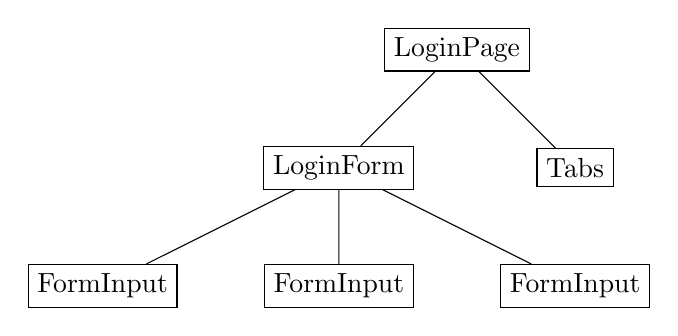
\begin{tikzpicture}[sibling distance=3cm, every node/.style = {draw, align=center}]
      
      \node {LoginPage}
        child { node {LoginForm} 
          child { node {FormInput} }
          child { node {FormInput} }
          child { node {FormInput} } }
        child { node {Tabs} };

    \end{tikzpicture}
    \caption{Component composition tree for the Login Page}
    \label{fig:login-components}
  \end{center}
\end{figure}

\begin{figure}[h!]
  \begin{center}
    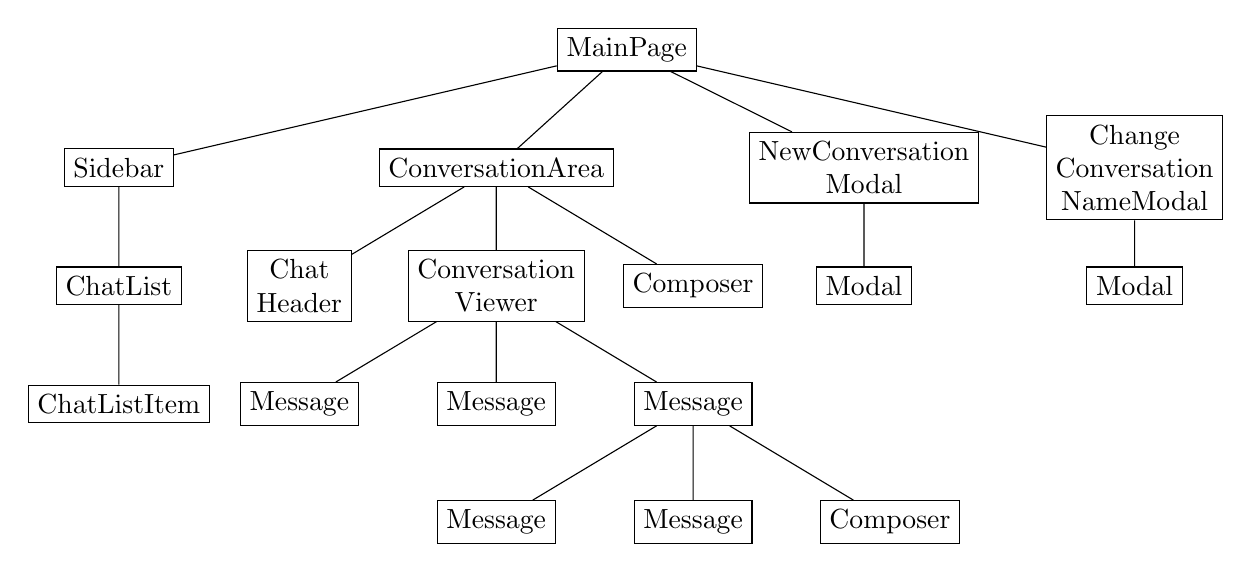
\begin{tikzpicture}[sibling distance=4.3cm, every node/.style = {draw, align=center}, level 2/.style={sibling distance=2.5cm}]
      
      \node {MainPage} 
        child { node {Sidebar} 
          child { node {ChatList} 
            child { node {ChatListItem} } } }
        child { node [right=-1cm] {ConversationArea} 
          child { node {Chat\\Header} }
          child { node {Conversation\\Viewer} 
            child { node {Message} }
            child { node {Message} }
            child { node {Message} 
              child { node {Message} }
              child { node {Message} }
              child { node {Composer} } } }
          child { node {Composer} } }
        child { node [right=-0.6cm] {NewConversation\\Modal} 
          child { node {Modal} } }
        child { node {Change\\Conversation\\NameModal}
          child { node {Modal} } };

    \end{tikzpicture}
    \caption{Component composition tree for the Main Page}
    \label{fig:main-components}
  \end{center}
\end{figure}

\subsection{Redux}
Redux has been used for application-level state management; that is, any state that is shared between and used by many different UI components in the application. The Redux model consists of a single Store, which contains the application state. The state is immutable, and the only way to update it is to emit an `Action', which describes what has happened on the UI, and can contain an optional data payload. In turn, `Reducers' are used to specify how the current state should be transformed, depending on which action is emitted. Reducers are pure functions which take the previous state and an action as parameters, and return the new state which is used to update the store \cite{redux-core-concepts}. The core concept of the Redux data flow is illustrated by Figure \ref{fig:redux-cycle} \cite{redux-implementation}.

\begin{figure}[h!]
  \begin{center}
    \begin{tikzpicture}[->,>=stealth',auto,node distance=3cm, minimum height=1cm, minimum width = 3cm, thick, main node/.style={rectangle, rounded corners, draw}]
    
      \node[main node] (1) [] {State};
      \node[main node] (2) [below right of=1, xshift=2.5cm] {UI};
      \node[main node] (3) [below left of=2, yshift=-0.5cm] {Actions};
      \node[main node] (4) [left of=3, xshift=-2cm] {Reducer};
      \node[main node] (5) [above left of=4, yshift=0.5cm] {Store};
    
      \path
        (1) edge node [above right] {defines} (2)
        (2) edge node [below right] {triggers} (3)
        (3) edge node [below] {sent to} (4)
        (4) edge node [below left] {updates} (5)
        (5) edge node [above left] {contains} (1);
    \end{tikzpicture}
    \caption{The Redux Flow}
    \label{fig:redux-cycle}
  \end{center}
\end{figure}

The use of Redux in this project provides a number of benefits. Firstly, since the key elements of Redux, actions and reducers, are just plain JavaScript objects and pure functions, respectively, unit testing becomes incredibly easy to perform without the need for complex mocking. Secondly, Redux removes the need for the React concept of `lifting state up', whereby state is kept in a high-level component, and is passed down to child components through \verb|props|. React code using this model becomes increasingly difficult to maintain, with state kept in different locations, and many components simply passing their props to their children without using them. Furthermore, since the state can only be updated by emitting an action, all changes to the state are centralised and happen one by one in a strict order; meaning that there are no race conditions to be aware of, the state is always predictable, and debugging is simplified \cite{redux-three-principles}.

To aid in software maintenance, the Redux reducer is split into separate functions, each of which is responsible for handling a separate `slice' of state, an example of functional decomposition. These reducers are then passed to the \verb|combineReducers()| function. The two separate slices of state handled by reducers in this application are `conversation' and `user'. The user reducer handles information about the currently logged in user, such as their email address; handling actions such as \verb|USER_LOGIN|. The conversation reducer is responsible for transforming the state regarding the conversations that are loaded from the mail server, handling many actions including \verb|SELECT_CONVERSATION|, \verb|LOAD_CONVERSATIONS|, and \verb|NEW_MESSAGE|.

\subsection{Improving Perceived Performance} % This section probably needs a better name......
When building the user interface, it was important to ensure that users' perceived the application as being fast and responsive, since this was one of the non-functional requirements. Activities such as sending emails, and fetching emails from IMAP mailboxes take some time, and by carefully considering user interface elements, the perceived time for these actions to be completed can be minimised.

Initially, the focus was placed on enhancing the user experience during fetching of messages from the mail server. It is suggested that loading spinners lead to a better perception of loading times than providing no animated feedback whatsoever \cite{persson2019improving}. Therefore a decision was made to implement loading spinners whilst waiting for the conversation info to be fetched immediately after login, and whilst waiting for messages to be fetched when a conversation is selected. Two animated loading indicators were implemented using the \verb|react-spinners| library \cite{react-spinners}, and these will ensure that users are aware that application is working in the background to load content and should increase perceived performance.

These loading spinners were present in the version of the application used in the first stage of User Acceptance Testing, and given the feedback from this testing, it would seem that they were largely effective. However, as is discussed in more detail in Section \ref{sec:stage1-uat}, many users found that the process of sending messages felt slow and unresponsive; to the extent that, in some cases, users sent messages multiple times because they thought that they had not initially been sent correctly. The reason for this poor user experience was due to the process that was used for adding sent messages to the user interface, which is illustrated in Figure \ref{fig:send-process}.

\begin{figure}[h!]
  \begin{center}
    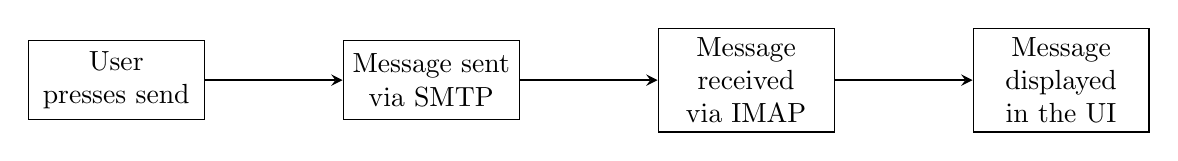
\begin{tikzpicture}[node distance=2cm]
      \tikzstyle{process} = [rectangle, minimum width=2cm, minimum height=1cm, text centered, text width=2cm, draw=black]
      \tikzstyle{arrow} = [thick,->,>=stealth]

      \node (press-send) [process] {User presses send};
      \node (smtp-send) [process, right of=press-send, xshift=2cm] {Message sent via SMTP};
      \node (imap-receive) [process, right of=smtp-send, xshift=2cm] {Message received via IMAP};
      \node (display) [process, right of=imap-receive, xshift=2cm] {Message displayed in the UI};

      \draw [arrow] (press-send) -- (smtp-send);
      \draw [arrow] (smtp-send) -- (imap-receive);
      \draw [arrow] (imap-receive) -- (display);
    \end{tikzpicture}
    \caption{Flowchart illustrating the message sending process}
    \label{fig:send-process}
  \end{center}
\end{figure}

In order to improve this user experience, changes were made to the message sending process. Under the modified process, as shown in Figure \ref{fig:new-send-process}, messages will be displayed in the UI as soon as they are sent, but with an additional `Sending' indicator. Once the message has been sent and then subsequently fetched from the mailbox, the stage at which the message would be shown under the original system, the sending indicator is removed.

\begin{figure}[h!]
  \begin{center}
    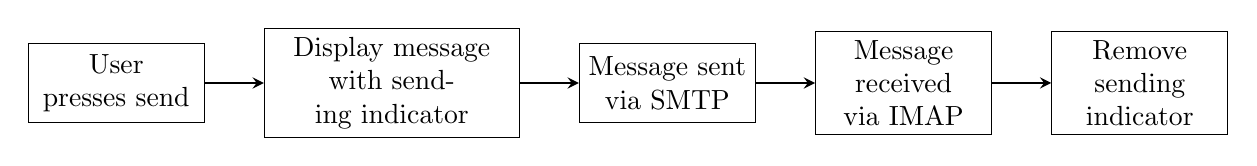
\begin{tikzpicture}[node distance=1cm]
      \tikzstyle{process} = [rectangle, minimum width=2cm, minimum height=1cm, text centered, text width=2cm, draw=black]
      \tikzstyle{arrow} = [thick,->,>=stealth]

      \node (press-send) [process] {User presses send};
      \node (display) [process, right of=press-send, xshift=2.5cm, text width=3cm] {Display message with sending indicator};
      \node (smtp-send) [process, right of=display, xshift=2.5cm] {Message sent via SMTP};
      \node (imap-receive) [process, right of=smtp-send, xshift=2cm] {Message received via IMAP};
      \node (update-ui) [process, right of=imap-receive, xshift=2cm] {Remove sending indicator};

      \draw [arrow] (press-send) -- (display);
      \draw [arrow] (display) -- (smtp-send);
      \draw [arrow] (smtp-send) -- (imap-receive);
      \draw [arrow] (imap-receive) -- (update-ui);
    \end{tikzpicture}
    \caption{Flowchart illustrating the message sending process}
    \label{fig:new-send-process}
  \end{center}
\end{figure}

\section{Service}

Aside from the user interface, the other core element of the application is the backend service, which is implemented as an Electron renderer process, but does not display a UI window. The service has two primary roles; firstly, to handle the sending of all email messages as required, and secondly, to handle the fetching of incoming emails from the mail server. These two sets of functionality are implemented independently of each other, and are orchestrated through a \verb|MailManager| object. A \verb|MailManager| object is instantiated when a user submits their login credentials, and is responsible for creating instances of the \verb|ImapClient| and \verb|SmtpClient| classes, which are discussed below in further detail. The \verb|MailManager| exposes methods which are called in response to IPC events from the frontend. The \verb|MailManager| is also responsible for registering event listeners to the \verb|ImapClient| object contained within it, to act upon events that are emitted, performing the necessary tasks in response.

% maybe put in a UML class diagram for the service here?

\subsection{Sending Email}
Emails are sent through the Simple Mail Transfer Protocol (SMTP) \cite{smtp-rfc} as this is the recognised standard for sending of email and is supported by all email providers. It was decided early in the implementation process that an existing library should be used to handle email sending, to avoid the complex and time-consuming task of building a client that implements the SMTP protocol from scratch based on the specification in RFC 5321 \cite{smtp-rfc}. The SMTP client is responsible for establishing a two-way transmission channel with a SMTP server, and transferring mail messages to that server for it to handle.

Research revealed two existing and maintained JavaScript libraries for sending email messages with SMTP. These are Nodemailer \cite{nodemailer} and smtp-client \cite{smtp-client}. The smtp-client library works at a relatively low-level, requiring each SMTP command to be manually invoked and sent to the server. It was decided that this low-level of control was not required for this project, and that the higher-level abstraction provided by Nodemailer would be more suitable.

To maintain a good level of separation of concerns within the code and to simplify access to library functions, all access to the nodemailer library is carried out through a dedicated class, \verb|SmtpClient|. This class handles the creation of a Nodemailer \verb|Transporter| instance, verification of account credentials, and sending of messages. It should be noted, however, that this class is not responsible for the construction of messages in-line with the schema defined for this application, to ensure that it is versatile and reusable. The generation of messages in the correct format is handled by separate parts of the codebase, and is discussed in Section \ref{sec:message-schema-implementation}.

\subsection{Receiving Email}
There are two protocols currently in use for accessing messages from mailboxes, IMAP \cite{imap-rfc} and POP3 \cite{pop-rfc}. The key difference between these two protocols is that when a client reads messages from the server using POP3, it downloads the messages, stores them locally, and removes them from the server. Using the IMAP protocol, messages are stored permanently on the server and are not removed unless unless explicitly deleted by the client. Based on the architecture of this application, whereby all messages are stored on the server, and fetched only when a conversation is loaded, it was immediately obvious that IMAP should be used for mailbox access in this project.

Preliminary research indicated two suitable libraries to simplify the use of IMAP in JavaScript. The first of these is node-imap \cite{node-imap} which allows programmatic access to an IMAP server, but works at a relatively low-level, requiring manual invocation of the commands used in the IMAP protocol. On the other hand, imap-simple \cite{imap-simple} is a wrapper around the node-imap library which provides a simplified programming interface. Due to the simplified interface, it was initially decided that imap-simple should be used in this project to speed up development time. As development of the software progressed, it became apparent that, since imap-simple ``is missing a great deal of functionality from node-imap'' \cite{imap-simple}, it was not going to be possible to use it in this application. Specifically, the problem with imap-simple was related to being able to use the \mintinline{js}{onmail} event listener that is invoked when new messages arrive in the mailbox. As a result, the underlying IMAP communications in this application are performed using node-imap.

Similar to the sending of email messages; a class, \verb|ImapClient|, has been implemented to ensure that interactions with the node-imap library are contained to one specific place in the code, to increase maintainability. It is important to note that the node-imap library makes extensive use of the Node.js event-driven programming model, emitting events when there is new data to respond to. The primary role of the \verb|ImapClient| class is to register listeners to the various events that are emitted by node-imap and ensure that the correct actions are performed in response. The class also provides methods which can be called to register new event listeners at runtime, based on specific events.

The node-imap library provides two key methods, \verb|search()| and \verb|fetch()|, which are used together to find and then download specific subsets of messages from the mail server. These methods allow for conditions to be applied to queries of the mail server, such as `unseen messages only' or `only messages with this subject'. After initiating a fetch, the messages found are emitted from the node-imap instance via events. In turn, these messages are transformed and collated by the ImapClient, before being emitted as events from the ImapClient itself, which is a subclass of \verb|EventEmitter|, to be handled by the MailManager.

IMAP inherently has a concept of 'SEEN' messages; a flag is set on the server for each message to denote whether a the message has been seen by the user or not \cite{imap-rfc}. When developing the methods to allow querying of the mailbox, it was important to consider under which circumstances messages should be marked as seen on the server. When messages are first received or are fetched when opening the application, their `SEEN' flag should not be modified. This ensures that messages which are marked as unread in the UI remain unread even if the application is closed and reopened. An exception to this is if a new message is received in the conversation that is currently open in the UI. In this case it is assumed that the message will have been read by the user and should therefore be marked as `SEEN'. Messages are also marked as `SEEN' when they are fetched as the result of a conversation being opened. 

Currently, the ImapClient class is also responsible for decrypting messages once they have been fetched from the server. Whilst this allowed for rapid development of a minimum viable product, ideally; under the principle of Single Responsibility of the SOLID design principles\cite{solid-principles}, the code for encryption and decryption should be in a separate module which can then be imported and used wherever necessary.

\subsection{Message Schema}\label{sec:message-schema-implementation}
Implementation of the message schemas designed in Section \ref{sec:message-schemas} is via a number of generation functions defined in \verb|threader.js|. These functions are exported from the module and utilised within the \verb|MailManager|. Messages are created by using the data passed to the generate functions as values in  JavaScript objects and these objects are then converted into JSON (JavaScript Object Notation) \cite{json-rfc} strings to be placed in the message body. 

As identified in the design stage, messages and conversations should both have unique IDs. This has been achieved through the use of Universally Unique Identifiers (UUIDs), specifically UUIDv4 \cite{uuid-rfc}. It was decided to use version 4 of UUID since it is based solely on random numbers, and since a namespace is not required as is the case in v3, it allowed for the simplest implementation.

It should be noted that these generation functions also generate the subject lines for messages, which include a tag identifying the messages as being either ordinary messages, or messages sent as one of the various stages of the key exchange process, as well as the message ID in the case of ordinary messages. The reasoning for putting the message ID in the subject of messages is to allow messages to be queried on the mail server quickly, without having to parse the entire message body. One important consideration that was taken into account when designing the subject format was the fact that each line of the subject should be no greater than 78 characters, excluding the \verb|CRLF| \cite{internet-message-format-rfc}. In order to keep the schema as simple as possible, it was decided that subjects should be only one line, and therefore the total length including the tag and the UUID, which have a fixed length of 36 characters \cite{uuid-rfc}, should be no more than 78, meaning that the tags were limited by design to 42 characters.